%\chapter{Methodology}
%\label{ch:methodology}
%why isn't the diamond growth section in here? fuck it, moving it. does it make more narrative sense? yeah I think so. Intro - ???semiconductor theory??? - diamond - metal contacts - 
\chapter{Diamond Growth and Devices/Characterisation}%/characteristaion? where the hell is this section going... basically methodology following literature review??? but where????
Or diamond dopants?

\label{ch:diamond}
\section{High Pressure High Temperature}
The high pressure high temperature (HPHT) method is one of the oldest and most well established methods for diamond synthesis. This process involves subjecting a carbon source such as graphite to conditions at which diamond becomes the stable form of carbon, typically 1400 to 1600 \si{\degreeCelsius} at pressures of 5 to 6 \si{\giga\pascal}. The high pressure and temperature allow the carbon atoms to rearrange into the crystal lattice structure of diamond. This is similar to the natural process of diamond growth, but accelerated with the metal catalyst to allow for mass production of diamonds, primarily for mechanical applications. 
\subsection{History}
Early efforts to produce synthetic diamond date back to the 19th century, with notable attempts by the French scientist Henri Moissan heating mixtures of iron and carbon in a reaction chamber to several thousand degrees Celcius, at high pressures. Diamonds were discovered following these experiments, but in 1962 it was revealed that the samples were natural in origin, perhaps detaching from the walls of the furnace.

Hence, true HPHT generated diamond was first developed in the 1950s, with scientists at General Electric, including Tracy Hall, discovering that diamond could be synthesised at high pressures and temperatures using metal catalysts in a "belt press" setup to apply the required conditions. Other notable figures in the development of the HPHT method include Robert Wentorf Jr., who was also at General Electric and made significant contributions to the development of the process.

The HPHT method has since been refined and is now used to mass-produce diamonds for various applications, including cutting and polishing, drilling, and as gemstones. Today, the global production of HPHT synthetic diamonds is estimated to be around 1.5 to 2 billion carats per year, with China, Russia, and the United States being the largest producers. While HPHT diamonds are mainly used for industrial applications, they are also increasingly being used as gemstones due to their high quality and clarity. The HPHT method has thus become an important tool for meeting the growing demand for diamonds.
\subsection{Dopants}

\section{Chemical Vapour Deposition}
Chemical vapour deposition (CVD) is a widely used method for diamond growth due to its ability to produce large, high-quality single crystals. The process involves the use of gas-phase precursors such as methane and hydrogen, which are introduced into a low-pressure reactor and excited to form a plasma above the substrates. The ratio of hydrogen to methane is a critical parameter for high-quality diamond crystal growth, as it affects the purity, morphology, and crystal quality of the resulting diamond film. A plasma is typically generated by microwave power in modern CVD chambers, but growth can also be achieved by methods such as hot filaments or blowtorches, which leads to the dissociation of the gas precursors and the generation of radicals or ions that allow for diamond crystal growth.

The growth process can be controlled using various parameters such as temperature, pressure, misorientation and gas flow rates. CVD diamond growth can be classified into two categories: homoepitaxy and heteroepitaxy. Homoepitaxy refers to the growth of diamond on a pre-existing diamond substrate such as that of a HPHT generated sample, while heteroepitaxy involves the growth of diamond on a substrate made of a different material. The use of non-diamond substrates presents challenges due to the large differences in thermal expansion coefficient and lattice constants, leading to defects and dislocations in the resulting diamond film.

In addition to the use of hydrogen and methane precursors, gases containing nitrogen, phosphorous, and boron can be added to the mixture to deliberately introduce impurities into the diamond lattice and alter its electrical and optical properties. 
\subsection{History}
CVD diamond growth has been intensively investigated as a method of producing synthetic diamond since the 1970's, with the first work by Derjaguin et al in 1975 demonstrating that it was possible to induce diamond growth in conditions of metastability with a heated substrate and cyclic growth/etching of graphitic material \cite{derjaguin:1975}. This was then developed by Spitsyn 1981 \cite{spitsyn:1981} and Nakazawa 1987 \cite{nakazawa:1987} into a more complete picture of homoepitaxial growth, with further refinements in more recent times.

Heteroepixial growth has been investigated from the onset of diamond growth too, with Spitsyn 1981 attempting to grow diamond layers on poly or single crystalline copper, silicon, tungsten, molybdenum and gold, with varying degrees of success. One of the most significant factors favouring the nucleation of diamond on foreign substrates is the suppression of graphite deposition while in the presence of atomic hydrogen. Kobashi 1988 \cite{kobashi:1988} investigated the usage of silicon substrates, with varying surface treatments such as micrometre diamond particle polishing to induce scratches. [Also Setaka 1984 in japanese?? Can't find this paper... in this area focus on using substrates with a lattice parameter which more closely resembles that of diamond, Yoshikawa 1990 cBN.... not homoepitaxy is it Koizumi??? Lee 1996 - nehanced nucleation density of chemical vapor deposition diamond by using interlayer looks good. ] Despite progress in heteroepitaxial growth, the lattice misfit of diamond on any substrate will cause significant strain to be induced in the grown layers. As a result, high quality, single crystalline CVD diamond on a variety is still a difficult prospect. 

%A massive discussion with jon on this... lots
\subsection{Growth Mechanisms}

\section{Dopants}
\label{section:diamond_doping}
\subsection{Incorporation Efficiency}
\label{subsection:incorporation_efficiency}
In studies examining the growth of n or p-type diamond, it is possible to consider the incorporation efficiency of the dopants involved. First, the density and molar mass of diamond are utilised to calculate the number of carbon atoms present in a cubic centimetre of diamond. With an approximate density of 3.51 \si{\gram\per\centi\metre\cubed} and a molar mass of 12.01 \si{\gram\per\mole}, the number of carbon atoms present can be calculated:
\begin{equation}
    \text{Number of carbon atoms per \si{\centi\metre\cubed}} = \left(\frac{\text{Density}}{\text{Molar mass}}\right)\times N_{A}
    \label{eq:incorporation_efficiency}
\end{equation}
Which results in $\approx1.76\times10^{23}$ \si{\atoms\per\centi\metre\cubed}. For simple reference, it is convenient to consider the magnitudes of phosphorous incorporation and their resulting atomic concentrations. Hence, incorporation efficiencies of 100\%, 10\%, 1\% and 0.1\% are used in the following sections in consideration of the doping concentrations. These efficiencies can then be considered for the various dopant:carbon sources for CVD growth. Naturally, it is unrealistic to consider the extreme cases in which there is no carbon source, but ratios of up to 50\% have been used to grow highly doped diamond films [\cite{kato2009,grotjohn2014}]. 

Therefore, as in \cite{koizumi1997}, diamond growth where there is a dopant:carbon ratio of 0.1\%, an incorporation ratio of 10\% results in approximately 0.01\% of the dopant being grown into the diamond lattice, corresponding to $0.01\times1.76\times10^{23}=1.76\times10^{19}$ \si{\atoms\per\centi\metre\cubed}. The actual measured concentration of dopant in this example had an incorporation efficiency of around 15\%, with the authors observing $2.5\times10^{19}$ \si{\atoms\per\centi\metre\cubed} of dopant as measured via SIMS analysis. 


\subsection{Nitrogen}
Substitutional nitrogen provides a "deep donor" in diamond, with an activation energy of around $1.6\si{\electronvolt}$. At room temperature then, this is more akin to a trapping state than than of a donor, with the material firmly within the freeze out region.

Adding a nitrogen source into the CVD process provides a growth rate enhancement \cite{dunst2009}.

\subsection{Boron}
Superconductors wow.

Kwak 2021 - A thorough review has been had, or at least a thorough read through. There are several papers that I need to follow up on, such as the equation for thermionic emission that has the current density as a variable and the fact that it is referencing several papers on SBD diamond... Which all seem very relevant to me nowadays.

\subsection{Phosphorous}
\label{subsection:phosphorous_doping}
Phosphorous isn't real, it's a lie from big diamond to make you think diamond is useful for devices.

Phosphorous doped diamond was first confirmed to have been grown via CVD in 1997 by Koizumi et al with a negative Hall coefficient at a measured carrier concentration of at least $2.5\times10^{19}$\si{\per\centi\metre\cubed} for 1000ppm of phosphine. Koizumi  Over the next decade, CVD growth of phosphorous doped diamond was explored in depth to produce lightly doped films with high electron mobilities such as that by Katagiri in 2004 at $10^{16}$\si{\per\centi\metre\cubed} with a Hall mobility of $660$\si{\centi\metre\squared\per\volt\per\second}.
\subsection{Other}
Sulphur (LOL).
\section{Surface Properties}
\subsection{Doped}
\subsection{Undoped}

\section{Luminescence of Diamond}

The energy which is emitted as photons from a material following the absorption of incident energy is broadly classed as luminescence. The exact form of luminescence varies based on the excitation energy, with photoluminescence due to the energy carried by photons, cathodoluminescence due to the absorption of energetic electrons (typically emitted from a cathode, hence the naming convention), and thermoluminescence by thermal excitation \cite{mei2015}.

Photoluminescence is then categorised based on the emission lifetime, which can either be relatively instantaneous, or delayed, with an emission lifetime that can span from tens of nanoseconds to hours or even days in specific circumstances. In the first case, colloquially defined as fluorescence, the luminescent centres release their stored energy immediately upon excitation, and the practical fluorescence lifetime of these centres is typically less than 50 nanoseconds. The second case is defined as phosphorescence, and this emission lifetime is well studied in diamond due to the variety of processes that can lead to such a delay between the absorption of energy and subsequent light emission \cite{li2016}.

\begin{figure}[h]
    \centering
    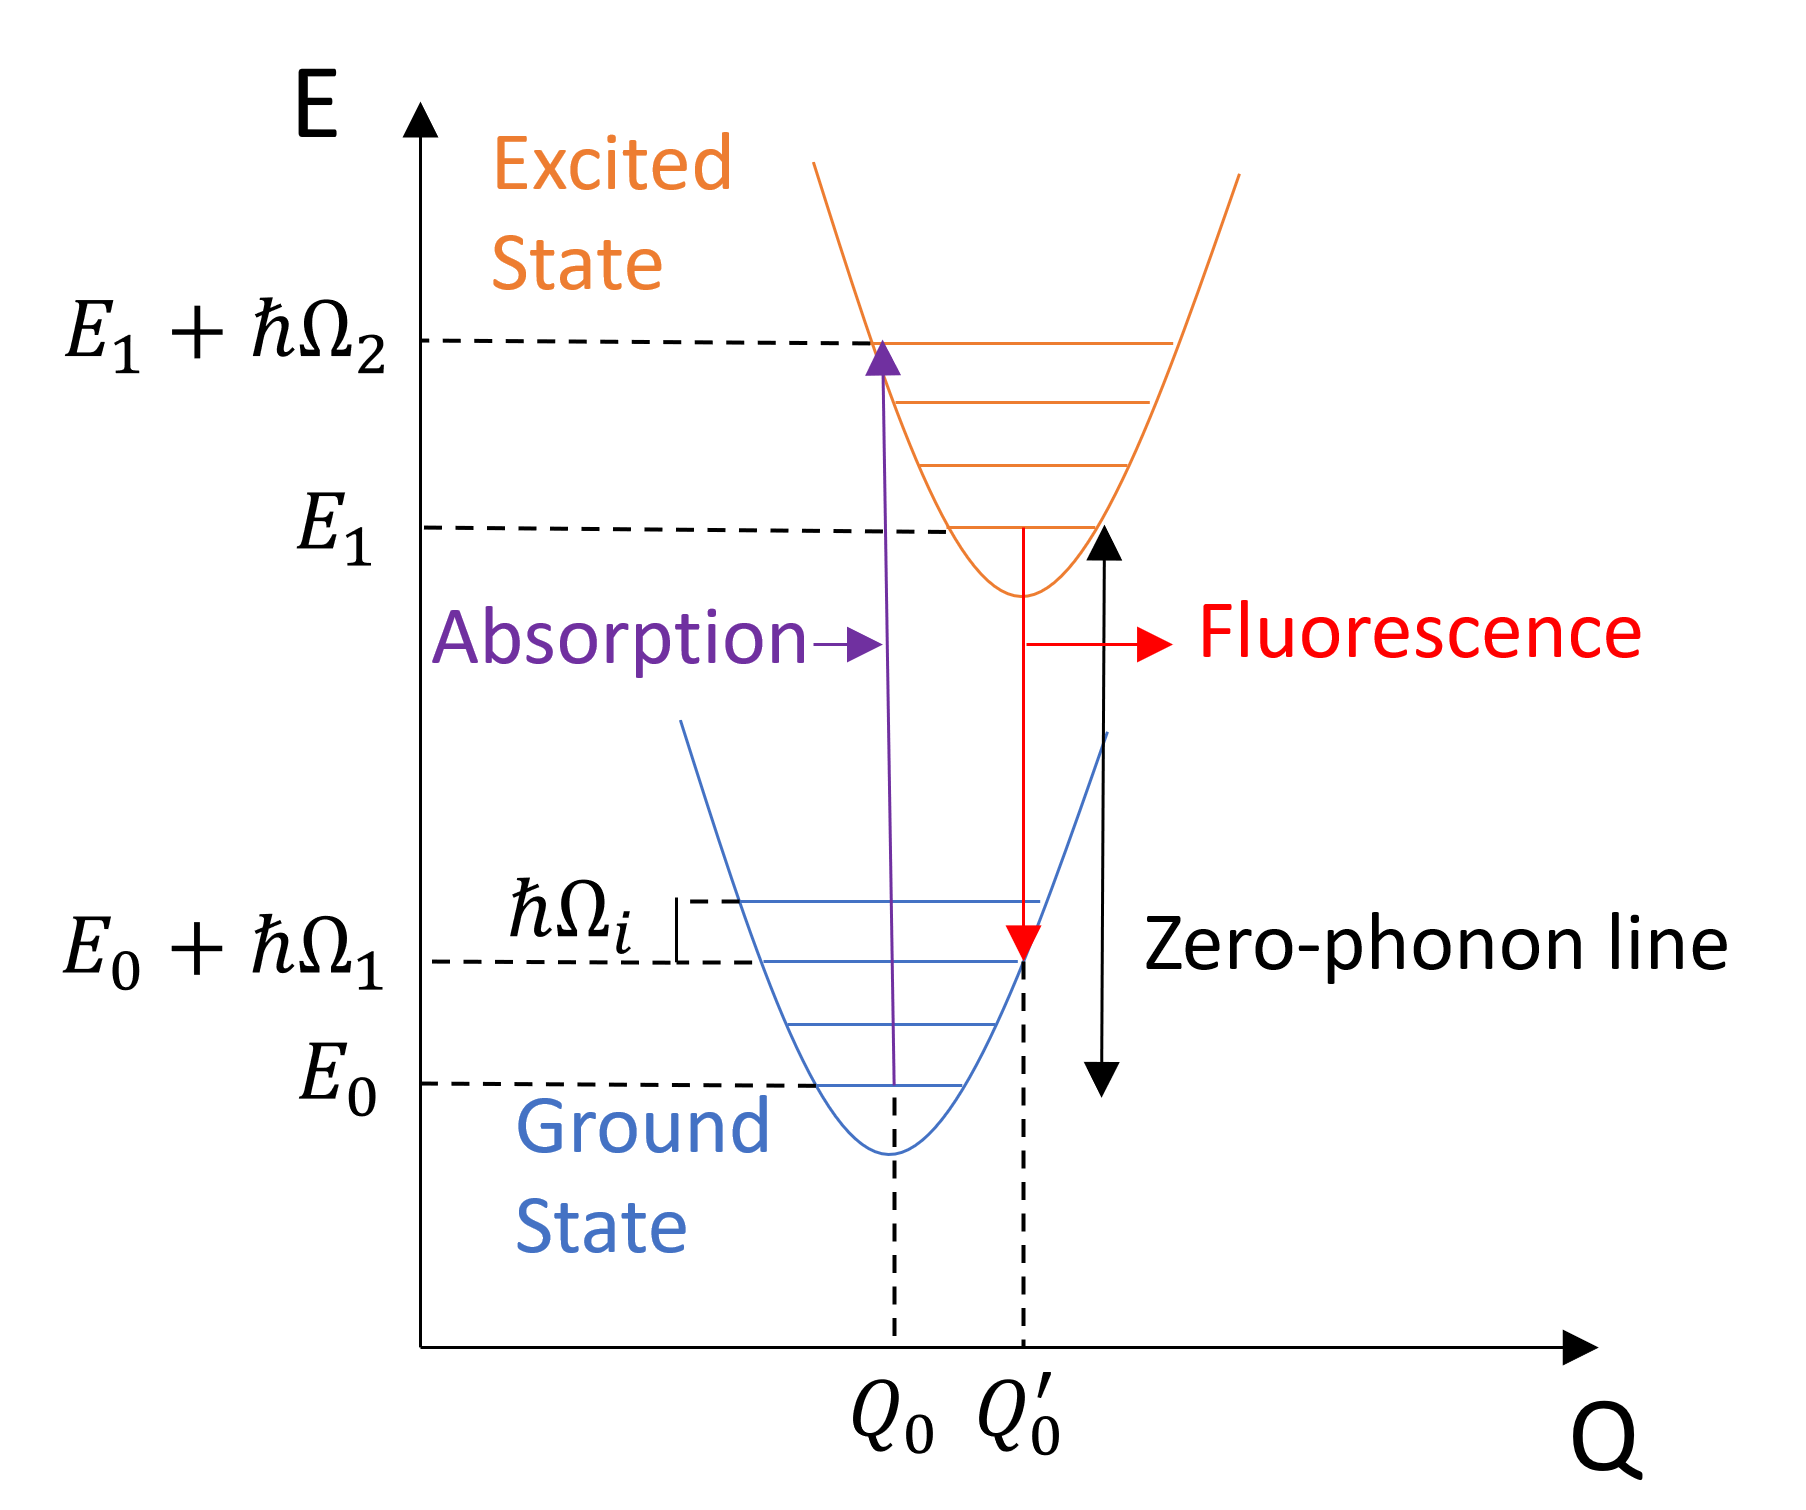
\includegraphics[width=0.6\textwidth]{Chapter3/Figs/Raster/fluorescence configuration diagram.png}
    \caption{Energy diagram for the ground state and an excited electronic state. $Q_{0}$ and $Q_{0}^{\prime}$ give the equilibrium positions of minimum value in the configuration coordinate for both the ground and excited states respectively.}
    \label{fig:fluorescence_diagram}
\end{figure}

Figure \ref{fig:fluorescence_diagram} provides a visual depiction of the processes involved in absorption and emission of energy in the form of fluorescence, against the configurational coordinate Q. Shown in this figure are the electronic transitions that are involved in such a process, with a system formed of electronic-vibrational interactions between states of impurities and the lattice vibrational modes. Absorption transitions in the vibronic system as shown are given by

\begin{equation}
    \hbar\omega_{a}=\left(E_{1} + \hbar\Omega_{2}\right)-E_{0}=\left(E_{1}-E_{0}\right)+\hbar\Omega_{1}.
    \label{eq:fl_diagram_absorption}
\end{equation}

Following the absorption of sufficient energy, the electron is then able to non-radiatively relax to the bottom of the excited state, with a radiative emission transition following this process of 

\begin{equation}
    \hbar\omega_{e} = E_{1}-\left(E_{0}+\hbar\Omega_{1}\right)=\left(E_{1}-E_{0}\right)-\hbar\Omega_{1}
    \label{eq:fl_diagram_emission}
\end{equation}
where the ground and excited electronic states are energy $E_{0,1}$ respectively, and $\Omega_{1,2}$ are the frequency of phonons created in the ground and excited state bands. Also included in figure \ref{fig:fluorescence_diagram} is the general characteristic vibrational energy difference between phonons $\hbar\Omega_{i}$. The transition between the ground and excited state is founded on the Franck-Condon principle, which states that the electronic transition is very fast compared to vibrational transitions, corresponding to motion within the crystal lattice. This is represented by the vertical transition lines within figure \ref{fig:fluorescence_diagram}, with no motion along the configurational coordinates during these transitions.

In the represented fluorescence transition, the emission energy is lower than that of the absorption, with the resulting red-shift generally termed the Stokes shift. The zero-phonon line (ZPL) is a noteworthy pure electronic transition between the lowest vibrational levels in both the ground and excited  states, and is observed as a sharp line with both the same frequency in absorption and emission spectrum. Electron-phonon coupling transitions tend to form continuous bands instead of discrete lines, due to the pairing of electronic states with multiple phonon modes. The transitions between two localised electronic states that are paired with differing phonon modes are called the phonon side-band (PSB). Equations \ref{eq:fl_diagram_absorption} and \ref{eq:fl_diagram_emission} show that the PSB is at higher energies than the ZPL when absorbing, and vice versa for emission, with the PSB giving lower energies when fluorescing due to the reduced change in electronic energy states. The ratio of PSB to ZPL differs based on the temperature, as the number of phonons in the lattice is temperature dependent.

\subsection{Optical Absorption}
While the diamond crystal structure itself is transparent from the start of shortwave UV-C at approximately 220 \si{\nano\metre} to the deep IR \cite{field2012}, crystalline defects are able to disrupt the lattice symmetry and produce weak dipole moments \cite{may1995}. These defects can then introduce extrinsic absorption features which are able to be used as spectral fingerprints of specific defects. Some of those absorption features may occur in the one-phonon mid-infrared region, such as for singly substitutional nitrogen which also has absorption patters in the visible region, and nitrogen aggregates which produce absorption in the UV area \cite{davies1976}, \cite{wang2004}, \cite{jones1992}. The resulting absorption coefficient is proportional to the density of optically obsorbing defects. This leads to the modern absorption spectroscopic analysis tools of Ultraviolet-visible absorption (UV-Vis absorption) or Fourier transform infra-red absorption (FTIR), which provide robust tools for investigating the characteristics of differing impurities and crucially, quantitative measurements of defect concentrations \cite{fadlelmoula2022}.

\section{Fabrication of Diamond Devices}
 The fabrication techniques for creating diamond-based devices involve processes such as photolithography, surface preparation or cleaning, metal deposition, and annealing. These techniques enable the creation of complex device geometries and contact patterns necessary for a variety of applications.
 
\subsection{Photolithography}
Photolithography is a process used in the manufacturing of integrated circuits (ICs) and micro electro-mechanical systems (MEMS) to transfer patterns onto a substrate. The basic process flow uses light and a photoresist, a light-sensitive material, to define and transfer patterns onto a substrate. The exact wavelength of light which is absorbed and the attenuation of light are parameters that can be tweaked, but it is typical for photoresist to react with UV light using the g-line (435 \si{\nano\metre}) or i-line (365 \si{\nano\metre}) of a mercuruy lamp in particular. Clean rooms for device manufacturing will then typically have yellow-tinted lights without any blue light component to avoid unintentional activation of the photoresist during the processing.

There are two types of photoresists used in photolithography: positive photoresists and negative photoresists, with the sign indicating the change in resist solubility when exposed to light of the correct wavelength. The choice between positive and negative photoresists depends on the requirements of the application, and both types of photoresist have their respective areas of usage.

\subsubsection{Positive}
Positive photoresists are photoresists that become more soluble in a developing solution when exposed to light. When a positive resist is used, the photoresist is first coated onto the substrate and then exposed to UV light through a mask, which is a patterned stencil that allows light to pass through specific areas and block it from others, in the shape of the desired pattern. The light exposed areas will become more soluble, so that when the substrate is immersed in a developer solution, the light exposed areas will wash away and leave behind a patterned photoresist with trenches leading down to the substrate in the areas where light exposure occurred.
Some of the advantages of a positive photoresist include:
\begin{itemize}
    \item Easy to process: They are easy to process, as they do not require the use of a post-exposure bake step, which is necessary for some negative photoresists.
    \item Good resolution: Positive photoresists can produce fine patterns with a high resolution.
    \item Good profile control: Positive photoresists will tend to form well defined patterns with straight sidewalls
\end{itemize}
Some disadvantages of positive photoresists include:
\begin{itemize}
    \item Limited shelf life: Positive photoresists have a limited shelf life and can degrade over time.
    \item Sensitivity to ambient light: Positive photoresists can be sensitive to ambient light and may require the use of light-tight containers to protect them from exposure.
\end{itemize}
% this is all shit. really quick zeroth draft crap churned out in like 5 minutes. COME BACK HERE AND DO IT AGAIN, THIS ALSO ISN'T RIGHT IS IT??? WELL MAYBE IT IS, BUT HOW DOES THIS FIT THE NARRATIVE STRUCTURE OF INTRO - DIAMOND/DEVICES THEORY - METHODOLOGY - METAL CONTACTS/NUMERICAL METHODS - COMPUTATIONAL WORK - EXPERIMENTAL WORK??? - CONCLUSIONS???? HOW DOES ANY OF IT FIT TOGETHER ACTUALLY NOW THAT i THINK ABOUT IT??? SURELY METAL CONTACTS/NUMERICAL METHODS COMES BEFORE METHODOLOGY? METHODOLOGY COULD THEN INCLUDE NUMERICAL METHODS AND SOME LEAD INTO THE COMPUTATIONAL STUFF??? BUT THEN THERE'S STILL A GAP BETWEEN METHODOLOGY AND EXPERIMENTAL WORK??? WHY IS MY CAPS LOCK ON HAVE A NICE DAY
\subsubsection{Negative}
Negative photoresists will generate the inverse of the pattern used for a positive photoresist, and hence are often referred to as "inversion" profiles". In a negative photoresist process, the photoresist is exposeed to light, which makes the exposed areas more resistant to a developer solution. When the substrate is then immersed in a developer solution, the unexposd areas are removed, leaving behind a patterned photoresist on the substrate.

Advantages of negative photoresists include:
\begin{itemize}
    \item Improved shelf life: Negative photoresists tend to have a longer shelf life and are less sensitive to degradation over time.
    \item Improved sensitivity: Negative photoresists are less sensitive to ambient light, which makes them more stable and easier to store.
    \item Improved patterning: Negative photoresist can produce more complex patterns with better edge acuity.
\end{itemize}
Some disadvantages of negative photoresists include:
\begin{itemize}
    \item More difficult to process: A post-exposure bake step is typically required, which is unnecessary for a positive photoresist.
    \item Lower resolution: Negative photoresists tend to produce patterns with poorer profile control and less defined sidewalls.
    \item Poorer profile control: Negative photoresists tend to produce patterns with poorer profile control and less defined sidewalls.
\end{itemize}

\section{Characterisation}
In the development of semiconductor devices, there are several key elements such as the sheet resistivity of semiconductors with various doping levels and metal-semiconductor junctions ranging from linear ohmic contacts with a low contact resistance to rectifying Schottky contacts of a high contact resistance. The fabrication of more complex devices hence requires reliable charactersiation techniques to determine the experimental values which will impact on device performance. This is especially true for wide bandgap semiconductors or diamond, where the crystalline quality and material properties as a result of doping with phosphorous is less well established.
\subsection{Current-Voltage (IV)}
Current-voltage (IV) measurements are a common method used to characterise the electrical properties of semiconductors such as silicon and wide bandgap materials like silicon carbide and gallium nitride. IV measurements involve applying a voltage to a device and measuring the resulting current flow. From this, the device's resistance, mobility, and other important electrical properties can be determined. One example of an IV measurement technique is the transfer length method (TLM). The TLM method involves fabricating a set of contacts of known dimensions on a sample, then measuring the current-voltage characteristics of the contacts to determine the resistance of the sample. The measured resistance is then used to calculate the specific contact resistance and sheet resistance of the sample. The TLM method is particularly useful for characterising high-resistivity materials, such as wide bandgap semiconductors, which are challenging to measure using other methods. In TLM measurements, rectangular or trapezoidal contact geometries are commonly used due to their ease of fabrication and ability to minimise parasitic effects. However, circular contacts are preferred due to the uniform current flow and lack of sharp edges, providing more accurate results, especially when the material is difficult to etch.
\subsection{Current-Voltage-Temperature (IVT)}
Current-Voltage-Temperature (IVT) measurements are able to provide a more complete picture of the electrical properties offered by metal contacts made to semiconductors than IV measurements alone. In addition to resistance and carrier mobilities, IVT measurements can also yield information about the activation energy of dopants, doping concentrations and carrier lifetimes of a sample. One common us of IVT measurements is the characterisation of Schottky barrier didoes, where the thermionic emission model is often used to describe the current flow across the metal-semiconductor interface. The thermionic emission model is typically given as:
[https://www.sciencedirect.com/science/article/pii/S1369800122000798] 2022 paper by efeoglu and turur for a nice full model with many references. Temp for now as lazy.
\begin{equation}
    I = A^* T^2 e^{-\frac{q\phi_B}{kT}}
    \label{eq:thermionic_emission_model_gpt}
\end{equation}
where $A^*$ is the Richardson constant, $T$ is the absolute temperature, $q$ is the elementary charge, $\phi_B$ is the Schottky barrier height, and $k$ is the Boltzmann constant. The saturation current:
\begin{equation}
    I_s = AT^2 e^{-\frac{q\phi_B}{kT}}
    \label{eq:thermionic_saturation_current}
\end{equation}
where $A$ is a device-specific constant that includes factors such as the effective area of the diode and the density of states of the semiconductor material.

The ideality factor:
\begin{equation}
    n = \frac{V_D}{kT/q}\ln\left(\frac{I_D}{I_s}\right)
    \label{eq:ideality_factor_thermionic}
\end{equation}
where $V_D$ is the voltage across the diode, $I_D$ is the diode current, and $k$, $T$, and $q$ have their usual meanings. The ideality factor $n$ is a measure of the deviation of the diode from the ideal thermionic emission model. A value of $n = 1$ indicates that the diode follows the thermionic emission model perfectly, while higher values of $n$ indicate the presence of additional current mechanisms, such as trap-assisted tunnelling or recombination.

\subsection{Atomic Force Microscopy}
First demonstrated in 1985 by Binnig, Quate and Gerber \cite{binnig:1986}, Atomic Force Microscopy (AFM) techniques are a high resolution non optical imaging technique that can be used to measure topographical, magnetic, electrical, optical, chemical and mechanical properties of sample surfaces in air, liquid or vacuum conditions. The accuracy, speed of data acquisition, non destructive measurements and relative low cost makes AFM techniques invaluable in labs worldwide.
\subsubsection{Principles of AFM Measurements}
A standard AFM system with optical feedback uses an AFM probe and sharp probe tip to scan the sample surface in a raster pattern \cite{marti:1999}. AFM tips are typically made of either silicon or silicon nitride, and are mounted on the end of a flexible cantilever, which has some reflective coating on the backside. The cantilever is mounted with a piezoelectric ceramic scanner, for precise control over both the lateral and vertical positions of the probe relative to the sample surface. As the AFM tip is scanned across a surface with topological features, the cantilever will deflect due to the slight change in vertical position. A laser beam is aimed at the back of the cantilever/probe tip, with the beam reflecting into a position sensitive photodetector. The slightest changes in deflection will cause a shift in the measured posititon of the laser spot, allowing for precise measurement of the deflection. In combination with the piezoelectric scanner, the change in height is accounted for via computer software to ensure that the tip will pass over hills and sink lower into trenches, while recording the 3D scan. This feedback loop maintains a constant interaction force, which will differ depending on the mode of AFM being used.

[Insert a small drawing maybe? nothing complicated just showing how the laser bounces off the cantilever and into the photodiode with the piezoscanner and sample surface.

The modes of operation are defined by the various regions of Van der Waals forces. When the probe tip is in "contact" mode, the force is repulsive and quite strong. In the "non-contact" mode, the probe tip experiences a milder, attractive force to the sample surface. Finally, the "tapping" mode will range from the attractive to the repulsive forces, as the probe tip oscillates from far away, to very close to the surface. These regions of the Van der Waals forces are shown in figure [another small drawing to make it clear].

%nanoandmore.com/what-is-atomic-force-microscopy for somewhat of a reference for the writing. Mostly coming from the top of my head on this front though which is nice
% just looked at this again and it's shit, check the top of your head because it's fuckin empty

\subsubsection{Contact}
When operated in "contact" mode, the AFM probe tip makes direct physical contact with the sample surface as it is scanned across the area of interest. This is defined by the tip experiencing a repulsive Van der Waals interaction with the surface. C-AFM is often used to measure the mechanical properties of materials, such as hardness, adhesion, and elastic modulus, as well as to image samples with a high degree of contrast, such as samples with large differences in height or stiffness. C-AFM can also be used for imagine samples in liquids or for imaging samples with large height differences, where the non contact mode is not feasible. However, contact mode AFM also has limitations, such as the potential for sample damage or measurement artifacts due to tip-sample interactions, and the difficulty of imaging delicate or soft samples.

The cantilever for a contact mode AFM probe needs to deflect easily without damaging the sample surface or tip. Hence, it is usually made to be very thin (0.3--2 \si{\micro\metre}), with a correspondingly low spring constant. The resonant frequency also needs to be high to avoid vibrational instability, so the length of the cantilever is made to be quite short (100--200\si{\micro\metre}). They are often shaped as a "V" to help provide a low resistance to vertical deflection while resisting lateral torsion.

\subsubsection{Non-Contact}
In non-contact mode, the probe tip experiences an attractive Van der Waals force with the sample surface, due to the increased separation. As this force is significantly lower than that of the attractive force experienced in contact mode, to resolve the minor deflections in the AFM cantilever an oscillation is induced. The relatively minor attractive force induces a change in the oscillation frequency, which is especially noticeable when the cantilever is oscillated at, or just above the resonant frequency. There are two common modes in usage, that of frequency modulation (FM) and amplitude modulation (AM). NC-AFM is useful for imaging delicate or sensitive samples,as well as for imaging samples with very high or very low surface energy, where direct contact with the tip would result in damage or measurement artifacts. NC-AFM is a powerful imaging technique, but it does have some disadvantages which include:
\begin{itemize}
    \item Imaging force limuitations: NC-AFM relies on the relatively weak attractive Van der Waals force, which can be sensitive to environmental factors, such as humidity, which can result in measurement artifacts or poor image quality.
    \item Limited imaging range: NC-AFM is limited in the range of sample heights that it can image due to the difficulty of maintaining a constant tip-sample separation. Samples with large height differences or steep slopes may be difficult to image with NC-AFM.
    \item Poor image contrast: NC-AFM typically provides images with lower contrast compared to contact mode atomic force microscopy as the imaging forces used are weaker and provide less information about the sample surface.
    \item High tip sensitivity: NC-AFM is highly sensitive to the tip and its environement, making it necessary to carefully control the tip and its surroundings to ensure consistent and accurate imaging.
    \item Low imaging speed: NC-AFM is typically slower than C-AFM as the tip must be kept at a constant separation from the sample during imaging, which can result in slower scan speeds and longer imaging times.
\end{itemize}
Despite these limitations, NC-AFM has many advantages, such as the ability to image delicate or sensitive samples without physical contact, making it a valuable tool in many applications. There are two different imaging modes which are used in NC-AFM, that of amplitude modulated (AM) and frequency modulated (FM) NC-AFM.
\paragraph{Amplitude Modulation}
In AM-NC-AFM, the tip is held at a constant height above the sample and the cantilever is oscillated at a frequency just above that of the resonant frequency. If the probe tip - sample surface separation decreases during a scan, then the tip will encounter the repulsive Van der Waals region, which then increases the resonant frequency of cantilever oscillation. As the separation increases, the attractive forces experienced by the tip will increase, which induces a decrease in the cantilever resonant frequency. This change in resonant frequency will cause singificant changes in the amplitude of oscillation as the tip is scanned across the surface of the sample, hence measurement of the cantilever amplitude allows for imaging of the surface profile.

The advantages of AM-NC-AFM when compared to FM include:
\begin{itemize}
    \item High sensitivity: AM is highly sensitive to small changes in the sample surface, making it useful for imaging delicate or soft samples.
    \item Low noise: AM has a low noise leve, which makes it possible to image samples with low signal to noise ratios.
\end{itemize}
Disadvantages of AM-NC-AFM:
\begin{itemize}
    \item Sensitivity to tip wear: AM is sensitive to tip wear, which can result in measurement artifacts or changes in the image quality over time.
    \item Poor image contrast: AM often provides images with lower contrast compared to FM, as the imaging forces used in AM are weaker and provide less information about the sample surface.
\end{itemize}

AM-AFM was one of the originally proposed modes in the 1986 paper \cite{binnig:1986}. The AFM cantilever is oscillated at a frequency just above that of the resonant frequency in this mode. As the probe tip is scanned over the surface, any attractive forces on the tip will cause a decrease in the overall probe resonant frequency, further reducing the amplitude of oscillation as the resonant frequency moves away from the driven oscillation. In contrast, when the tip moves closer to the surface and experiences a repulsive force due to the tip proximity, the resonant frequency of the cantilever will increase, approaching the driven oscillation frequency and hence increasing the resultant amplitude of oscillation. This shift is shown in figure [drawing from the AFM handbook which I drew months back to understand it]. The computer system can then translate the measured amplitude into a measured topographical height, either in the feedback loop of 
\paragraph{Frequency Modulation}
First developed by Albrecht, Gr{\"u}tter, Horne and Rugar in 1991, this mode tracks the changes in the resonant frequency of AFM cantilever.
FM-NC-AFM uses a frequency modulation approach, where the resonant frequency of the cantilever is monitored as the tip is scanned across the sample, rather than the amplitude of the oscillation.

Advantages of FM when compared to AM-NC-AFM include:
\begin{itemize}
    \item High image contrast: FM provides high contrast images, as the samples interaction with the tip results in large changes in the resonant frequency, which provides more information about the sample surface.
    \item Robustness: FM is robust against tip ear, as the measurement is based on changes in the resonant frequency, which are less sensitive to tip wear compared to changes in oscillation amplitude.
\end{itemize}
Disadvantages of FM:
\begin{itemize}
    \item Limited sensitivity: FM is less sensitive compared to AM, as the measurement is based on changes in the resonant frequency, which are less sensitive to small changes in the sample surface.
    \item High noise: FM has a high noise level, which can make it difficult to image samples with low signal to noise raios
\end{itemize}

\paragraph{Comparison of AM to FM}
In conclusion, AM and FM NC-AFM each have their own advantages and disadvantages, with the choice between the two modes depending on the specific requirements of the imaging task.
\subsubsection{Tapping / Dynamic Force}
Dynamic force microscopy (DFM) is so named as it is a type of AFM in which the dynamic interaction between a probe and sample is measured. The probe is oscillated at its resonant frequency, and the interaction force between the probe and sample is measured by the changes in the oscillation amplitude or phase of the probe. This allows for a more sensitive measurement of the sample's surface properties, such as stiffness, adhesion, and friction. The oscillation between repulsive and attractive Van der Waals can also be thought of as physical tapping of the surface, with the probe at the very edge of the attractive and repulsive forces.

Compared to contact AFM, DFM provides a higher level of sensitivity, as it is able to measure the dynamic interaction between the probe and sample. This allows for imaging of softer and more delicate samples, as well as the ability to probe the mechanical properties of the sample.

However, there are also some disadvantages to DFM. One disadvantage is that it requires a high level of stability and control in the oscillation of the probe, as small variations in the oscillation can affect the measurement. Additionally, the measurement is more sensitive to environemental factors, such as temperature, humidity, and air currents, which can affect the stability of the probe's oscillation. Hence, while DFM provides several advantages as a blend of both contact and non-contact AFM measurements, it also has some disadvantages that must be taken into account. The choice of the best AFM technique depends on the type of sample, the information desired and the level of precision and sensitivity required.

When operated in tapping mode, the cantilever needs to have a higher spring constant to reduce imaging noise and instabilities. They are typically made to be rectangular in shape, in contrast to the contact V shapes.  
\subsection{Helium Ion Microscopy}
\label{subsec:him}
Helium ion microscopy (HIM) is a type of imaging technology that uses a focused beam of helium ions to create high-resolution images of a sample. It can be compared to scanning electron microscopy (SEM), which is a similar, commonly used technique to scan samples, with some important differences.

First, HIM uses a beam of helium ions, while SEM uses a beam of electrons. The helium ions in HIM have a much smaller wavelength than electrons, which enable HIM to achieve higher resolution than SEM. The resolution of an imaging technique can be calculated using the Rayleigh criterion, which states that the minimum resolvable distance between two points is equal to the width of the point-spread function (PSF) of the imaging system. The PSF is a function that describes how the imaging system responds to a point source. For HIM and SEM, the PSF can be modelled as a Gaussian distribution with a standard deviation given by:

\begin{equation}
    \sigma = \frac{0.61\lambda}{NA}
    \label{eq:PSF_standard_deviation}
\end{equation}

where $\lambda$ is the wavelength of the probe (either helium ions for HIM or electrons for SEM), and NA is the numerical aperture of the objective lens. The numerical aperture is a measure of the lens' ability to collect light or particles from the samples. Assuming a helium ion beam with a wavelength of $0.05\si{\nano\metre}$ and a numerical aperture of $0.1$, the standard deviation of the PSF for HIM can be calculated as:

\begin{equation}
    \sigma = \frac{0.61*0.05 \si{\nano\metre}}{0.1} = 0.305 \si{\nano\metre}
    \label{eq:PSF_HIM_standard_deviation}
\end{equation}

for comparison, assuming an electron beam with a wavelength of $0.2\si{\nano\metre}$ and a numerical aperture of $0.1$, the standard deviation of the PSF for SEM can be calculated as:

\begin{equation}
    \sigma = \frac{0.61*0.2\si{\nano\metre}}{0.1} = 1.22 \si{\nano\metre}
    \label{eq:PSF_SEM_standard_deviation}
\end{equation}

therefore, the PSF for HIM is much smaller than that of SEM, resulting in higher resolution imaging. In addition, the helium ions in HIM interact more weakly with the sample than electrons int SEM, leading to less sample damage and higher quality imaging.

Overall, the smaller wavelength and weaker interaction of helium ions with the sample in HIM result in better resolution and less sample damage compared to SEM.
\subsection{Raman Microscopy}
\label{subsec:raman_microscopy}
Raman microscopy is a technique uesd for chemical analysis and imaging of samples. It is based on the Raman scattering phenomenon or Raman effect, which is a type of inelastic scattering of light, which occurs when light interacts with the vibrational or rotational modes of a molecule. In the Raman effect, the molecule absorbs a photon of light, which excites it to a virtual energy state. The molecule then emits a scattered photon, which has a different frequency and energy than the incident photon. The frequency and energy difference between the incident and scattered photons is equal to the vibrational or rotational energy of the molecule. 

The Raman effect can be understood in terms of the polarisability of the molecule. The polarisability of a molecule is a measure of its ability to be polarised by an electric field. In the Raman effect, the interaction between the incident light and the molecule causes a temporary polarisation of the molecule, which leads to the emission of scattered light.


\subsection{Fluorescence Microscopy}% this is really needing a review and rewrite... a single day of effort could probably vastly expand on this. I need to explain why this is significant for the laser written devices etc etc. give a short lit review on the published characterisation techniques yadayada


Fluorescence is widely used in a variety of fields due to the applications which result from this phenomena, and 

The second case of delayed luminescence is then known as 

Fluorescence microscopy is a type of optical microscopy that uses fluorescence to introduce contrast in the imaging of either samples or biological specimens. Fluorescence is a property of certain molecules that emit light of a different colour or wavelength when they are excited by light of a specific wavelength. In fluorescence microscopy, a fluorescent molecule is attached to the specimen, or the specimen itself is made fluorescent by adding a fluorophore. The physics behind fluorescence can be understood in terms of the electronic structure of molecules and the laws of quantum mechanics, and applies to both the biological fluorophores as well as 

In a molecule, electrons are arranged in distinct energy levels, with the lowest energy level being the ground state. When a molecule absorbs a photon of light, the energy of the photon is transferred to one of the electrons, causing it to move to a higher energy level. This excited state is unstable, and the electron will eventually return to the ground state, releasing the absorbed energy in the form of a photon of light. The energy of the emitted photon is lower than that of the absorbed photon, and the difference in energy is released as heat or other forms of energy. The emitted light is typically in the visible range and can be detected using a variety of techniques.